\section{Results}
\begin{figure}[ht]
    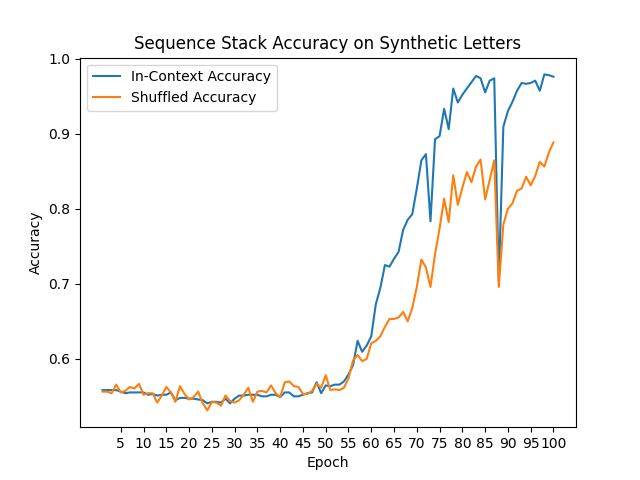
\includegraphics[width=0.5\textwidth]{figures/sequence_stack_mnist_like.png}
    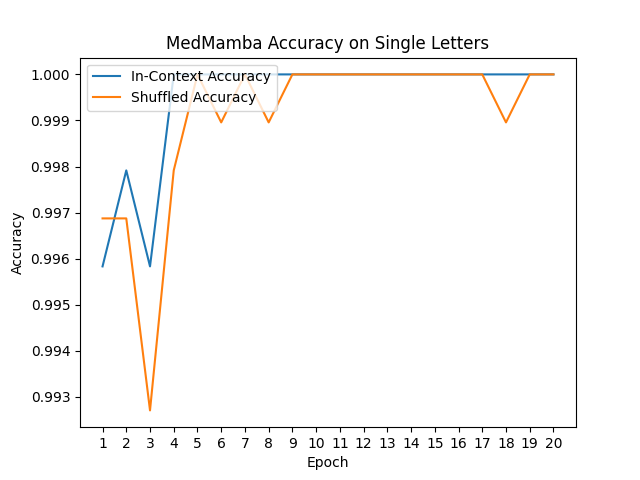
\includegraphics[width=0.5\textwidth]{figures/medmamba_mnist_like.png}
    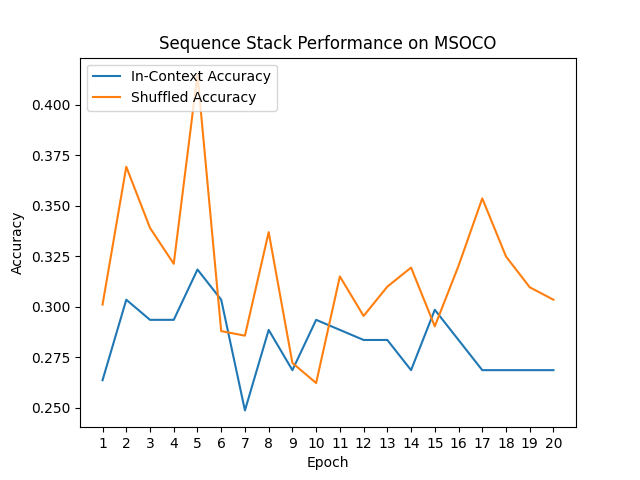
\includegraphics[width=0.5\textwidth]{figures/sequence_stack_mscoco.png}
    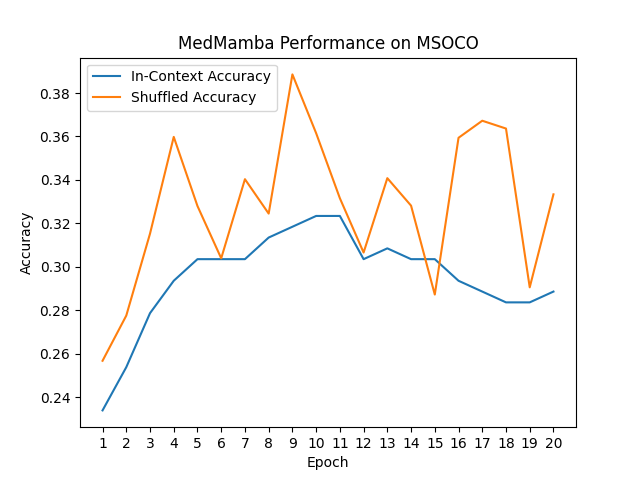
\includegraphics[width=0.5\textwidth]{figures/medmamba_mscoco.png}
    \caption{Graphs of results}
    \label{resultslide}
\end{figure}
In our tests with synthetic data, we found that our in-context learning
hypothesis is confirmed. With single-character context images, we find that
in-context predictions are significantly more accurate compared to predictions
in shuffled contexts.

However, with multi-character tasks we find that performance degrades
significantly. In addition, the in-context accuracy boost disappears.
We suspect that this degradation is due to memory limitations within Mamba;

This effect also appears with the synthetic dataset, so it is unlikely that this
effect is due to poor data quality.

One possible explanation is that the multi-character task requires multi-engram
correlation.
This is a task that Mamba performs very poorly on\cite{mambangram}.
Thus, it could be possible that Mamba layers's finite memorization capability
is being used on memorizing actual characters as opposed to memorizing fonts
and colors.

It's also important to note that with multi-character tasks, the distance
between the correlates is variable.
this might pose a challenge to Mamba, as it would have to also map the correct
characters in sequence to the correct label tokens.
This is likely to be a much harder task for Mamba.

